\subsection{Declaration Graph}\label{app:decl-detail}

\subsubsection{Declaration Kinds}

\begin{table}[ht]
\centering
\caption{Declaration kinds in $G_{\mathrm{thm}}$: role, prevalence, and representative example.}
\label{tab:kind-overview}
\small
\begin{tabular}{lp{5.2cm}rrl}
\toprule
Kind & Role & Count & \% & Example \\
\midrule
theorem     & Proved proposition; proof erased at runtime   & $243{,}725$ & $79.1$ & \decl{Nat.add\_comm} \\
definition  & Computable function; body retained            & $48{,}664$  & $15.8$ & \decl{List.length} \\
abbrev      & Transparent shorthand; always unfolded        & $6{,}667$   & $2.2$  & \decl{OfNat.ofNat} \\
constructor & Introduction rule of an \texttt{inductive}    & $4{,}755$   & $1.5$  & \decl{Nat.succ} \\
inductive   & New type with introduction rules              & $3{,}813$   & $1.2$  & \decl{Nat} \\
opaque      & Sealed body; cannot be unfolded               & $499$       & $0.2$  & \decl{Float.add} \\
quotient    & Kernel primitives for quotient types          & $3$       & ${<}0.1$ & \decl{Quot.mk} \\
axiom       & Accepted without proof; irreducible           & $3$       & ${<}0.1$ & \decl{propext} \\
\bottomrule
\end{tabular}
\end{table}

\subsubsection{Inter-Kind Edge Flow}

\begin{table}[H]
\centering
\caption{Inter-kind edge flow in $G_{\mathrm{thm}}$. Each row is a source kind; each column is a target kind. Entries are thousands of edges; blanks denote fewer than $500$.}
\label{tab:inter-kind-flow}
\small
\begin{tabular}{l*{5}{r}}
\toprule
Source $\downarrow$ \textbackslash\ Target $\rightarrow$ & theorem & definition & abbrev & inductive & \textit{other} \\
\midrule
theorem      & $1{,}332$k & $2{,}498$k & $2{,}590$k & $835$k & $241$k \\
definition   & $18$k      & $285$k     & $284$k     & $163$k & $50$k \\
abbrev       & $2$k       & $17$k      & $26$k      & $20$k  & $3$k \\
constructor  & $1$k       & $12$k      & $20$k      & $16$k  & $6$k \\
inductive    &            & $2$k       & $3$k       & $6$k   & $5$k \\
axiom/opaque/quotient &   & $1$k       &            &        & \\
\bottomrule
\end{tabular}
\end{table}

\subsubsection{Degree Statistics by Declaration Kind}

\begin{table}[ht]
\centering
\caption{Degree statistics by declaration type. In-degree measures how often a declaration is cited; out-degree measures how many premises it invokes.}
\label{tab:thm-kind-degree}
\small
\begin{tabular}{lrrrrrrrrr}
\toprule
& & \multicolumn{4}{c}{In-degree} & \multicolumn{4}{c}{Out-degree} \\
\cmidrule(lr){3-6} \cmidrule(lr){7-10}
Kind & Count & Mean & Med.\ & Max & Std & Mean & Med.\ & Max & Std \\
\midrule
axiom       & $3$       & $7{,}823$ & $169$ & $23{,}226$ & $10{,}892$ & $0.7$ & $1$ & $1$ & $0.5$ \\
abbrev      & $6{,}667$ & $438$     & $11$  & $89{,}936$ & $3{,}033$  & $10.0$ & $7$ & $106$ & $10.8$ \\
inductive   & $3{,}813$ & $273$     & $31$  & $44{,}487$ & $1{,}541$  & $4.1$ & $3$ & $54$ & $4.4$ \\
constructor & $4{,}755$ & $59$      & $7$   & $69{,}580$ & $1{,}104$  & $11.7$ & $8$ & $127$ & $10.9$ \\
definition  & $48{,}664$& $58$      & $4$   & $62{,}942$ & $739$      & $16.4$ & $13$ & $146$ & $13.7$ \\
theorem     & $243{,}725$& $5.5$   & $1$   & $58{,}686$ & $237$      & $30.8$ & $21$ & $522$ & $31.2$ \\
quotient    & $3$       & $305$     & $226$ & $596$      & $213$      & $0.3$ & $0$ & $1$ & $0.5$ \\
opaque      & $499$     & $0.5$     & $0$   & $21$       & $1.4$      & $3.9$ & $3$ & $33$ & $3.1$ \\
\bottomrule
\end{tabular}
\end{table}

\subsubsection{Zero-Citation Rates by Namespace}

\begin{table}[ht]
\centering
\caption{Zero-citation rates by namespace (extremes among namespaces with $\ge 100$ theorems).}
\label{tab:thm-leaves}
\small
\begin{tabular}{lrrrlrrr}
\toprule
\multicolumn{4}{c}{Highest zero-citation rate} & \multicolumn{4}{c}{Lowest zero-citation rate} \\
\cmidrule(lr){1-4} \cmidrule(lr){5-8}
Namespace & Total & Zero & Rate & Namespace & Total & Zero & Rate \\
\midrule
\ns{AddEquiv}           & $129$  & $119$ & $92.2\%$ & \ns{Primrec}            & $133$ & $17$ & $12.8\%$ \\
\ns{EMetric}            & $192$  & $163$ & $84.9\%$ & \ns{AnalyticAt}         & $102$ & $15$ & $14.7\%$ \\
\ns{DomMulAct}          & $105$  & $89$  & $84.8\%$ & \ns{AkraBazziRecurrence}& $129$ & $21$ & $16.3\%$ \\
\ns{Ordering}           & $127$  & $105$ & $82.7\%$ & \ns{ContinuousWithinAt} & $119$ & $20$ & $16.8\%$ \\
\ns{LocallyConstant}    & $113$  & $93$  & $82.3\%$ & \ns{HasFDerivWithinAt}  & $120$ & $21$ & $17.5\%$ \\
\ns{MulEquiv}           & $243$  & $194$ & $79.8\%$ & \ns{ConvexOn}           & $111$ & $20$ & $18.0\%$ \\
\ns{AddSubgroup}        & $111$  & $88$  & $79.3\%$ & \ns{LipschitzWith}      & $113$ & $21$ & $18.6\%$ \\
\ns{AddMonoidHom}       & $138$  & $108$ & $78.3\%$ & \ns{DifferentiableAt}   & $113$ & $21$ & $18.6\%$ \\
\bottomrule
\end{tabular}
\end{table}

\subsubsection{Edge Classification}

\begin{table}[ht]
\centering
\caption{Edge classification in $G_{\mathrm{thm}}$ by module and namespace relationship.}
\label{tab:thm-edge-breakdown}
\begin{tabular}{lrr}
\toprule
Category & Edges & Percentage \\
\midrule
Same module                    & $811{,}649$   & $9.6\%$ \\
Cross-module, same namespace   & $805{,}772$   & $9.6\%$ \\
Cross-namespace                & $4{,}296{,}412$ & $50.9\%$ \\
Missing module info            & $2{,}522{,}533$ & $29.9\%$ \\
\bottomrule
\end{tabular}
\end{table}

\subsubsection{Cross-Namespace Pairs}

\begin{table}[ht]
\centering
\caption{Top~10 cross-namespace edge pairs in $G_{\mathrm{thm}}$, ordered by edge count.}
\label{tab:thm-cross-ns-pairs}
\small
\begin{tabular}{llr}
\toprule
Namespace A & Namespace B & Edges \\
\midrule
\ns{AlgebraicGeometry}  & \ns{CategoryTheory}    & $38{,}042$ \\
\ns{CategoryTheory}     & \ns{Quiver}            & $29{,}286$ \\
\ns{CategoryTheory}     & \ns{Eq}                & $27{,}927$ \\
\ns{CategoryTheory}     & \ns{HomologicalComplex} & $15{,}829$ \\
\ns{MeasureTheory}      & \ns{Real}              & $15{,}668$ \\
\ns{MeasureTheory}      & \ns{Set}               & $11{,}954$ \\
\ns{MeasureTheory}      & \ns{ProbabilityTheory} & $11{,}734$ \\
\ns{Eq}                 & \ns{MeasureTheory}     & $10{,}385$ \\
\ns{Complex}            & \ns{Real}              & $10{,}370$ \\
\ns{ENNReal}            & \ns{MeasureTheory}     & $10{,}302$ \\
\bottomrule
\end{tabular}
\end{table}

\subsubsection{Extended Analysis}\label{app:decl-analysis}

\noindent\textit{1. The double infrastructure.}\\
The hub structure of $G_{\mathrm{thm}}$ decomposes into two layers that the module graph conflates: a \emph{language infrastructure} layer (\decl{OfNat.ofNat}, \decl{Eq.refl}, \decl{DFunLike.coe}) determined by Lean's type system, and a \emph{mathematical infrastructure} layer (\decl{CategoryTheory.Category}, \decl{Real}, \decl{TopologicalSpace}) determined by the logical structure of formalized mathematics (Remark~\ref{rem:two-layers}). This separation is invisible at the module level, where both layers cohabit the same source files. The language layer is a trace of the process---the specific proof assistant chosen---embedded in the product.

\medskip
\noindent\textit{2. Disciplinary autonomy as emergent community structure.}\\
Louvain community detection recovers seven major mathematical disciplines from the dependency topology alone (Table~\ref{tab:thm-communities}), with a modularity of $0.48$. The alignment with namespace organization, however, is only moderate (NMI $= 0.34$, ARI $= 0.18$; Table~\ref{tab:thm-nmi}). Among the major namespaces, only \ns{CategoryTheory} achieves near-complete community correspondence ($97.4\%$ concentration in a single community), suggesting that it is a genuinely autonomous mathematical discipline within \module{Mathlib}---self-contained in its dependency structure to a degree that no other branch achieves. All other communities are cross-namespace mixtures, confirming that the dependency topology discovers a structure related to, but distinct from, the human-imposed namespace hierarchy.

\medskip
\noindent\textit{3. The depth of cross-disciplinary entanglement.}\\
The cross-namespace edge density of $G_{\mathrm{thm}}$ ($50.9\%$; Table~\ref{tab:thm-edge-breakdown}) far exceeds that of $G_{\mathrm{module}}^{-}$ ($37.1\%$; \S\ref{sec:cross-namespace}). This gap reveals that module-level analysis \emph{underestimates} the true extent of mathematical interdependence. Module boundaries bundle cross-namespace theorem dependencies into single intra-directory import edges, creating an illusion of disciplinary containment that dissolves at finer granularity.

\paragraph{Contingency of hub structure.}
The hub rankings raise a question that our data can frame but not resolve: to what extent does the hub structure reflect the intrinsic logical architecture of mathematics, and to what extent does it reflect the contingent path by which human contributors developed the library? The mathematical infrastructure layer plausibly reflects genuine mathematical centrality: these concepts would remain foundational regardless of who proved the theorems. But the language infrastructure layer is an artifact of Lean's type system, and its prominence would differ under a different proof assistant. Between these two layers lies a gray zone: the specific \emph{ordering} in which theorems were formalized, and the specific \emph{lemma decomposition} that human provers chose, may have created hub concentrations that a different development history would not produce. Distinguishing intrinsic mathematical centrality from path-dependent formalization artifacts remains an open problem.

\medskip

Table~\ref{tab:thm-vs-module} summarizes the key quantitative contrasts between the two levels of analysis.

\begin{table}[ht]
\centering
\caption{Module-level ($G_{\mathrm{module}}$) vs.\ theorem-level ($G_{\mathrm{thm}}$) comparison.}
\label{tab:thm-vs-module}
\begin{tabular}{lrr}
\toprule
Metric & $G_{\mathrm{module}}$ / $G_{\mathrm{module}}^{-}$ & $G_{\mathrm{thm}}$ \\
\midrule
Nodes                        & $7{,}563$          & $308{,}129$ \\
Edges                        & $23{,}570$ / $19{,}448$ & $8{,}436{,}366$ \\
Cross-namespace edges         & $37.1\%$           & $50.9\%$ \\
In-degree max                & $167$              & $89{,}936$ \\
Community--namespace NMI     & ---                & $0.34$ \\
Single-node removal impact   & $29$ components    & $\le 6$ nodes disconnected \\
Zero-citation nodes          & $1{,}433$ sources  & $109{,}088$ leaf theorems ($44.8\%$) \\
\bottomrule
\end{tabular}
\end{table}

The theorem--premise graph is a more direct projection of the logical product than the module graph: its hubs, communities, and cross-namespace flows are less contaminated by file-organization conventions. Yet even at this finer resolution, the process leaves indelible traces in the product. The language infrastructure layer (Remark~\ref{rem:two-layers}) records the design choices of Lean's type system---a different proof assistant would produce a different in-degree ranking, even for the same mathematics. The $44.8\%$ leaf theorem rate (Remark~\ref{rem:leaf-theorems}) includes a substantial fraction of \texttt{@[to\_additive]} mirrors---a process-level automation that inflates the graph's surface without deepening its logical content. The out-degree distribution's lognormal shape (Remark~\ref{rem:thm-degree-asymmetry}) encodes a cognitive constraint: the bounded complexity of proofs that humans can construct or that tactics can synthesize. Even in the most product-like graph we have analyzed, the process is not erased; it is encoded.

For AI premise selection systems, the two-layer hub structure suggests a practical preprocessing step: filtering language-infrastructure premises (which carry no mathematical content) from training data may improve the signal-to-noise ratio. The theorem/lemma distinction, recoverable from source code (\S\ref{sec:thm-vs-lemma}), provides an additional human-annotated importance signal that could inform premise ranking.

\subsubsection{Degree Distribution}
\label{sec:thm-degree}

The degree statistics of $G_{\mathrm{thm}}$ reveal a striking asymmetry between the two directions of dependency.

\begin{table}[ht]
\centering
\caption{Degree statistics for $G_{\mathrm{thm}}$.}
\label{tab:thm-degree}
\begin{tabular}{lrr}
\toprule
Statistic & In-degree & Out-degree \\
\midrule
Mean    & $27.38$    & $27.38$ \\
Median  & $1$        & $19$ \\
Std Dev & $620.10$   & $29.18$ \\
Max     & $89{,}936$ & $522$ \\
Zero-degree nodes & $119{,}633$ & $367$ \\
\bottomrule
\end{tabular}
\end{table}

The in-degree distribution has median~$1$ but mean~$27$ and standard deviation~$620$---a ratio of standard deviation to mean exceeding~$22$, indicating extreme concentration. A handful of declarations accumulate tens of thousands of citations while the majority are referenced at most once. The out-degree distribution, by contrast, has median~$19$, standard deviation~$29$, and maximum~$522$---a far more concentrated profile.

To test whether these distributions follow a power law, we apply the Clauset--Shalizi--Newman method (\S\ref{sec:prelim-powerlaw}).

\begin{table}[ht]
\centering
\caption{Power law fit and distribution comparisons for $G_{\mathrm{thm}}$. The likelihood ratio $R > 0$ favors power law; $R < 0$ favors the alternative. A $p$-value below $0.05$ indicates a statistically significant comparison.}
\label{tab:thm-powerlaw}
\begin{tabular}{lrrrr}
\toprule
& \multicolumn{2}{c}{In-degree} & \multicolumn{2}{c}{Out-degree} \\
\cmidrule(lr){2-3} \cmidrule(lr){4-5}
Metric & Value & $p$ & Value & $p$ \\
\midrule
$\alpha$ (exponent)     & $1.781$ & --- & $2.936$ & --- \\
$x_{\min}$              & $20$    & --- & $38$    & --- \\
$\sigma$ (std.\ error)  & $0.005$ & --- & $0.008$ & --- \\
Tail fraction           & $11.1\%$ & --- & $20.6\%$ & --- \\
\midrule
vs.\ Lognormal ($R$)          & $-2.48$   & $0.174$   & $-1{,}452.5$ & $\approx 0$ \\
vs.\ Exponential ($R$)        & $+28{,}766$ & $\approx 0$ & $-239.9$ & $0.014$ \\
vs.\ Stretched Exp.\ ($R$)    & $+105.8$  & $\approx 0$ & $-1{,}495.9$ & $\approx 0$ \\
vs.\ Truncated Power Law ($R$) & $-21.5$  & $\approx 0$ & $-1{,}509.5$ & $\approx 0$ \\
\bottomrule
\end{tabular}
\end{table}

For in-degree, the tail ($k \ge 20$, comprising $11.1\%$ of non-zero values) is well described by a heavy-tailed distribution with exponent $\alpha \approx 1.78$. Pure power law decisively beats exponential and stretched exponential alternatives, but a \emph{truncated power law} provides a significantly better fit ($R = -21.5$, $p \approx 0$), and the comparison with lognormal is inconclusive ($p = 0.17$). This pattern---heavy tail, uncertain between power law and lognormal, best fit by a truncated power law---is characteristic of many real-world networks~\cite{clauset2009}.

For out-degree, the picture is categorically different: \emph{every} alternative distribution significantly outperforms pure power law. The best fits are lognormal and truncated power law, both with overwhelmingly negative likelihood ratios.

\noindent\textbf{Note.}
\label{rem:thm-degree-asymmetry}
This asymmetry has a structural explanation that connects directly to the central tension of the paper. In-degree measures how often a declaration is \emph{cited}---a cumulative, open-ended quantity determined by the logical structure of the completed library (the product). There is no upper bound: \decl{OfNat.ofNat} can be cited by any proof that involves a numeral, and its in-degree ($89{,}936$) reflects a form of preferential attachment in which foundational declarations attract ever more dependents. Out-degree, by contrast, measures how many premises a single proof \emph{invokes}---a quantity bounded by the cognitive and logical complexity of that proof (the process). No human-written proof cites $90{,}000$ lemmas; the maximum out-degree of~$522$ reflects the practical ceiling of proof complexity. The in-degree distribution records the product; the out-degree distribution records the process.

\begin{figure}[ht]
\centering

\includegraphics[width=\textwidth]{figures/thm_degree_distribution.pdf}
\caption{Degree distributions of $G_{\mathrm{thm}}$ on log--log axes. Left: in-degree, with power law fit (gold line, $\alpha = 1.78$, $x_{\min} = 20$). Right: out-degree. The in-degree tail extends over four orders of magnitude; the out-degree distribution is sharply bounded.}
\label{fig:thm-degree}
\end{figure}

\noindent\textbf{Transitive reduction at the theorem level.}
\label{rem:thm-transitive-reduction}
In contrast to the module graph, where transitive reduction removes $17.5\%$ of edges (\S\ref{sec:transitive-reduction}), the theorem--premise graph does not admit a meaningful transitive reduction. In $G_{\mathrm{module}}$, redundant edges arise from deliberate human choices---developers importing umbrella modules for cognitive convenience. In $G_{\mathrm{thm}}$, every edge is extracted mechanically from the proof term by the kernel: if a premise appears in the proof, the edge exists, regardless of whether that premise could be reached indirectly through other premises. The distinction is significant: module-level redundancy measures the gap between what the compiler requires and what the human chooses; at the theorem level, this gap vanishes, because the data already records exactly what the compiler sees.

\subsubsection{DAG Depth}
\label{sec:thm-dag-depth}

$G_{\mathrm{thm}}$ is a DAG with $84$ topological layers---roughly half the depth of $G_{\mathrm{module}}$'s $154$ layers. This compression is counterintuitive: the finer-grained graph has \emph{fewer} vertical layers. The explanation lies in transitivity. Each module-level layer spans multiple files that import each other; at the declaration level, the dependencies within those files are resolved in parallel rather than sequentially. The result is a shallower but vastly wider structure: the source layer alone contains $119{,}633$ declarations ($38.8\%$ of all nodes)---these are declarations with zero in-degree, i.e., declarations that no other declaration cites. By contrast, only $401$ declarations are sinks (zero out-degree).

\begin{figure}[ht]
\centering

\includegraphics[width=\textwidth]{figures/thm_dag_structure.pdf}
\caption{DAG width by topological layer for $G_{\mathrm{thm}}$ ($84$ layers). The source layer ($119{,}633$ zero-citation declarations) dominates; the remaining layers decay rapidly, reaching single digits by layer~$60$.}
\label{fig:thm-dag-structure}
\end{figure}

The extreme asymmetry between sources and sinks reflects the zero-citation phenomenon noted in \S\ref{sec:thm-degree}: nearly $39\%$ of declarations are never cited by another declaration. These terminal leaves populate layer~$0$ and give the declaration-level DAG its characteristic top-heavy profile.

\subsubsection{Centrality}
\label{sec:thm-centrality}

In \S\ref{sec:centrality}, we found that in-degree, PageRank, and betweenness centrality identify different structural roles at the module level. We now compute the same three measures on $G_{\mathrm{thm}}$ and find that the divergence between them is, if anything, more extreme.

\begin{table}[ht]
\centering
\caption{Top~10 declarations by in-degree, PageRank ($\alpha = 0.85$), and betweenness centrality (sampled, $k = 500$) in $G_{\mathrm{thm}}$.}
\label{tab:thm-centrality}
\small
\begin{tabular}{rlrlrl}
\toprule
\multicolumn{2}{c}{In-degree} & \multicolumn{2}{c}{PageRank} & \multicolumn{2}{c}{Betweenness} \\
\cmidrule(lr){1-2} \cmidrule(lr){3-4} \cmidrule(lr){5-6}
$\deg^{-}$ & Declaration & PR & Declaration & $c_B$ & Declaration \\
\midrule
$89{,}936$ & \decl{OfNat.ofNat}       & $.0151$ & \decl{CT.Category.mk}    & $.000338$ & \decl{Real} \\
$69{,}580$ & \decl{Eq.refl}           & $.0145$ & \decl{OfNat.mk}           & $.000338$ & \decl{Real.ofCauchy} \\
$65{,}437$ & \decl{DFunLike.coe}      & $.0140$ & \decl{outParam}           & $.000289$ & \decl{Rat.linearOrder} \\
$63{,}530$ & \decl{Membership.mem}    & $.0125$ & \decl{OfNat}              & $.000256$ & \decl{Real.pi} \\
$62{,}942$ & \decl{Eq.mpr}            & $.0123$ & \decl{CT.Category}        & $.000253$ & \decl{Real.$\exists$cos\_eq\_0} \\
$59{,}997$ & \decl{Set}               & $.0106$ & \decl{Eq.refl}            & $.000183$ & \decl{Rat.instIsStrictOrd.} \\
$58{,}686$ & \decl{Eq.trans}          & $.0097$ & \decl{Quiver}             & $.000177$ & \decl{Rat.le\_refl} \\
$56{,}019$ & \decl{Semiring.toNAR}    & $.0095$ & \decl{Quiver.mk}          & $.000164$ & \decl{Real.zero\_lt\_one} \\
$48{,}801$ & \decl{of\_eq\_true}      & $.0084$ & \decl{LE}                 & $.000157$ & \decl{Complex.log} \\
$48{,}295$ & \decl{PO.toPreorder}     & $.0084$ & \decl{LE.mk}              & $.000155$ & \decl{instSemiringNNReal} \\
\bottomrule
\end{tabular}
\end{table}

\noindent
\textit{Abbreviations:} CT = CategoryTheory, NAR = NonAssocSemiring, PO = PartialOrder, instIsStrictOrd.\ = instIsStrictOrderedRing, $\exists$cos\_eq\_0 = exists\_cos\_eq\_zero.

\medskip

The three columns of Table~\ref{tab:thm-centrality} have almost no overlap, and each tells a different story about the structure of \module{Mathlib}.

\emph{In-degree} is dominated by language infrastructure. The top entries---\decl{OfNat.ofNat}, \decl{Eq.refl}, \decl{DFunLike.coe}, \decl{Membership.mem}, \decl{Eq.mpr}---are type-class coercions and equality constructors that the elaborator inserts into virtually every proof term. Their prominence reflects the design of Lean~4, not the structure of mathematics. This contrasts with the module-level in-degree ranking (Table~\ref{tab:centrality}), where the top entry (\module{Mathlib.Init}) is a file that every module must import; the underlying mechanism---implicit foundational dependency---is analogous, but the theorem level reveals the specific \emph{declarations} responsible.

\emph{PageRank} promotes a different set of nodes: the constructors and types of category theory (\decl{CategoryTheory.Category.mk}, \decl{Quiver}, \decl{Quiver.mk}) and core algebraic infrastructure (\decl{OfNat}, \decl{LE}, \decl{Zero}). The key divergence from in-degree is \decl{CategoryTheory.Category.mk}: it ranks first in PageRank but does not appear in the in-degree top~$20$. Its PageRank reflects not its direct citation count but the fact that the entire $59{,}724$-node category theory subgraph depends on it transitively. PageRank captures \emph{recursive} importance---it identifies the foundations on which large, internally coherent subgraphs rest.

\emph{Betweenness centrality} reveals a third, entirely disjoint set of structurally critical declarations. The top entries---\decl{Real}, \decl{Real.ofCauchy}, \decl{Rat.linearOrder}, \decl{Real.pi}, \decl{Real.exists\_cos\_eq\_zero}---trace the construction chain of the real numbers. These nodes sit at the narrow passage connecting the algebraic world (rational numbers, ordered rings, number fields) to the analytic world (measure theory, complex analysis, probability). \decl{Real.pi} occupies rank~$4$ because $\pi$'s definition threads through number theory, trigonometry, and analysis, making it a crossroads of multiple mathematical disciplines. Only $34{,}564$ of $308{,}129$ nodes ($11.2\%$) have nonzero betweenness, confirming that shortest paths through $G_{\mathrm{thm}}$ are concentrated through a small number of critical bridges.

Figures~\ref{fig:thm-centrality-indeg-pr}--\ref{fig:thm-centrality-betw-pr} visualizes the pairwise relationships between the three centrality measures.

\begin{figure}[H]
\centering
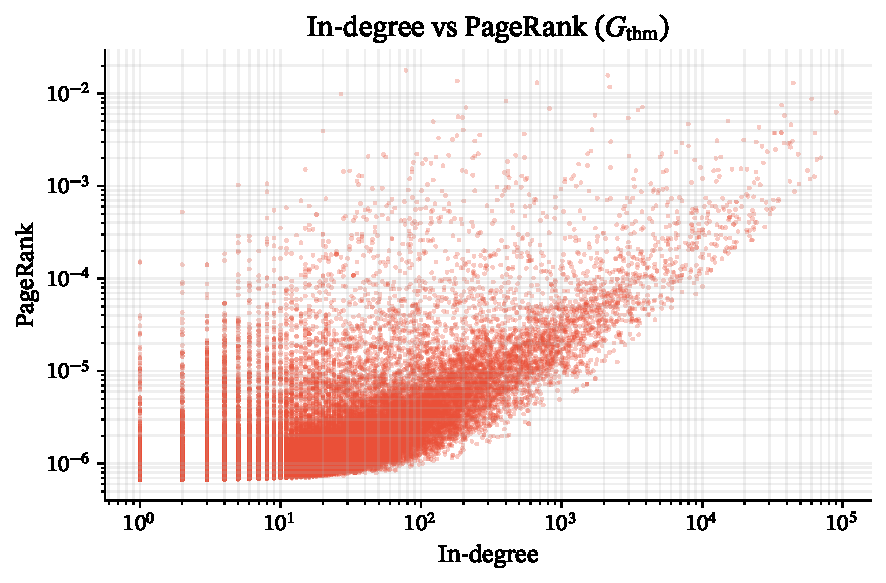
\includegraphics[width=\textwidth]{figures/thm_centrality_indeg_pr.pdf}
\caption{In-degree vs.\ PageRank in $G_{\mathrm{thm}}$. Each point is one declaration. The wide scatter confirms that popularity (in-degree) and influence (PageRank) measure different structural properties at the declaration level.}
\label{fig:thm-centrality-indeg-pr}
\end{figure}

\begin{figure}[H]
\centering

\includegraphics[width=\textwidth]{figures/thm_centrality_indeg_betw.pdf}
\caption{In-degree vs.\ betweenness centrality in $G_{\mathrm{thm}}$. Declarations with high betweenness but moderate in-degree act as bottleneck connectors between proof clusters.}
\label{fig:thm-centrality-indeg-betw}
\end{figure}

\begin{figure}[H]
\centering

\includegraphics[width=\textwidth]{figures/thm_centrality_betw_pr.pdf}
\caption{Betweenness vs.\ PageRank in $G_{\mathrm{thm}}$. The three-way divergence is not confined to the top-$10$ extremes but pervades the entire distribution, confirming that no two centrality measures are redundant.}
\label{fig:thm-centrality-betw-pr}
\end{figure}

\noindent\textbf{Note.}
\label{rem:thm-centrality-vs-module}
The three-way divergence of centrality measures observed at the module level (\S\ref{sec:centrality}) intensifies at the theorem level: no declaration appears in all three top-$10$ lists of Table~\ref{tab:thm-centrality}. The taxonomy of importance proposed in \S\ref{sec:module_conclusion}---\emph{vocabulary} (in-degree), \emph{axiomatic core} (PageRank), \emph{structural bridges} (betweenness)---receives sharper instantiation here. At the module level, the centrality rankings are partially confounded by file-organization artifacts (e.g., \module{Mathlib.Init} ranks high in all three measures simply because it is imported by every file). At the theorem level, these artifacts are stripped away, and the three measures separate cleanly into language infrastructure (in-degree), mathematical foundations (PageRank), and inter-disciplinary bridges (betweenness).

\subsubsection{Community Structure}
\label{sec:thm-community}

We apply Louvain community detection (\S\ref{sec:prelim-community}) to the largest weakly connected component of $G_{\mathrm{thm}}$ (converted to an undirected graph, $308{,}054$ nodes, $8{,}431{,}648$ undirected edges).

\begin{table}[ht]
\centering
\caption{Community detection summary for $G_{\mathrm{thm}}$.}
\label{tab:thm-community-summary}
\begin{tabular}{lr}
\toprule
Metric & Value \\
\midrule
Number of communities & $22$ \\
Modularity & $0.4757$ \\
Communities with ${>}1{,}000$ nodes & $7$ \\
Communities with ${>}100$ nodes & $11$ \\
\bottomrule
\end{tabular}
\end{table}

The modularity of $0.48$ indicates a moderately strong community structure---significantly above random ($0$) but below perfectly modular ($1$). If logical dependency alone determined community structure (pure product), modularity would be higher; if cognitive organization were independent of logic (pure process), it would approach zero. The intermediate value quantifies the partial---but incomplete---alignment between mathematical necessity and human practice. The $22$ communities are highly unequal: seven communities of more than $1{,}000$ nodes account for $99.1\%$ of the graph; the remaining fifteen communities contain fewer than $700$ nodes each.

\begin{table}[ht]
\centering
\caption{The seven major communities of $G_{\mathrm{thm}}$ (Louvain, $> 1{,}000$ nodes), with size, dominant mathematical theme, and top representatives by PageRank.}
\label{tab:thm-communities}
\small
\begin{tabular}{rrllp{4cm}}
\toprule
ID & Size & Theme & Top namespace(s) & Representatives \\
\midrule
0  & $63{,}763$ & Order / Sets / Filters & \ns{Set}, \ns{Filter}, \ns{Matroid} & \decl{LE}, \decl{Set}, \decl{Iff.intro}, \decl{Zero} \\
5  & $59{,}724$ & Category Theory & \ns{CategoryTheory} (69\%) & \decl{CT.Category.mk}, \decl{Quiver}, \decl{CT.CategoryStruct} \\
2  & $54{,}649$ & Algebra & \ns{LinearMap}, \ns{Matrix}, \ns{Module} & \decl{outParam}, \decl{Zero.mk}, \decl{Semiring} \\
1  & $49{,}739$ & Combinatorics / Discrete & \ns{List}, \ns{Finset}, \ns{SimpleGraph} & \decl{OfNat.mk}, \decl{Eq.refl}, \decl{List.nil} \\
11 & $38{,}245$ & Number Theory / Polynomials & \ns{Nat}, \ns{Int}, \ns{Polynomial} & \decl{OfNat}, \decl{Mul}, \decl{Semiring.mk} \\
7  & $37{,}368$ & Analysis / Probability & \ns{MeasureTheory}, \ns{Real} & \decl{Real}, \decl{MeasurableSpace} \\
8  & $2{,}773$ & Model Theory / Set Theory & \ns{FirstOrder}, \ns{SetTheory} & \decl{FirstOrder.Language.mk} \\
\bottomrule
\end{tabular}
\end{table}

These seven communities map recognizably onto traditional mathematical subdisciplines. The alignment is not imposed by the analysis; it emerges from the dependency topology alone. Louvain knows nothing about mathematical content---it optimizes modularity on the undirected edge structure---yet it recovers divisions (algebra vs.\ analysis, category theory vs.\ combinatorics) that correspond to centuries-old disciplinary boundaries.

To quantify the alignment between community structure and the namespace hierarchy, we compute the Normalized Mutual Information (NMI) and Adjusted Rand Index (ARI, Definition~\ref{def:nmi}--\ref{def:ari}) between two labelings of the $308{,}054$ nodes: the Louvain community assignment and the top-level namespace extracted from each declaration's module path.

\begin{table}[ht]
\centering
\caption{Alignment between Louvain communities and top-level namespaces.}
\label{tab:thm-nmi}
\begin{tabular}{lrl}
\toprule
Metric & Value & Interpretation \\
\midrule
NMI & $0.3432$ & Moderate association \\
ARI & $0.1817$ & Weak-to-moderate agreement \\
\bottomrule
\end{tabular}
\end{table}

The moderate NMI and low ARI confirm that dependency topology and namespace organization are \emph{related but far from identical}. The most striking case is \ns{CategoryTheory}: $97.4\%$ of its $42{,}094$ declarations fall into Community~$5$, and conversely, $68.7\%$ of Community~$5$ belongs to the \ns{CategoryTheory} namespace. This near-perfect correspondence is unique among the major communities. By contrast, the largest community (Community~$0$, $63{,}763$ nodes) draws its largest namespace contribution from root-level declarations ($17.1\%$), followed by \ns{Set} ($8.1\%$) and \ns{MeasureTheory} ($4.6\%$)---no single namespace dominates.

\noindent\textbf{Note.}
\label{rem:nmi-tension}
The NMI of $0.34$ provides a theorem-level metric for the tension between the module tree $T$ and the logical dependency graph $G$, extending the cross-namespace analysis of \S\ref{sec:cross-namespace}. At the module level, $37.1\%$ of reduced import edges cross namespace boundaries; at the theorem level, the NMI of $0.34$ quantifies the same phenomenon from a complementary angle---the dependency-based community structure aligns only moderately with the human-imposed namespace hierarchy. These two measures converge on the same conclusion: cognitive classification and logical structure are correlated but distinct, and the gap between them widens as granularity increases.

The exceptional case of category theory deserves emphasis. Its near-complete community--namespace alignment ($97.4\%$) suggests that category theory is not merely a namespace convention but a genuinely \emph{autonomous} mathematical discipline within \module{Mathlib}---its internal dependency structure is dense enough to form a self-contained community with minimal need for external foundations beyond the shared core. No other major namespace achieves this degree of self-containment.

\begin{figure}[H]
\centering

\includegraphics[width=\textwidth]{figures/community_decl_graph.pdf}
\caption{Louvain community aggregation graph of $G_{\mathrm{thm}}$ (modularity~$= 0.48$). Communities below $1\%$ of nodes are merged into ``Other''. \ns{CategoryTheory} and \ns{MeasureTheory} form the two largest communities.}
\label{fig:community-decl-graph}
\end{figure}

\begin{figure}[H]
\centering
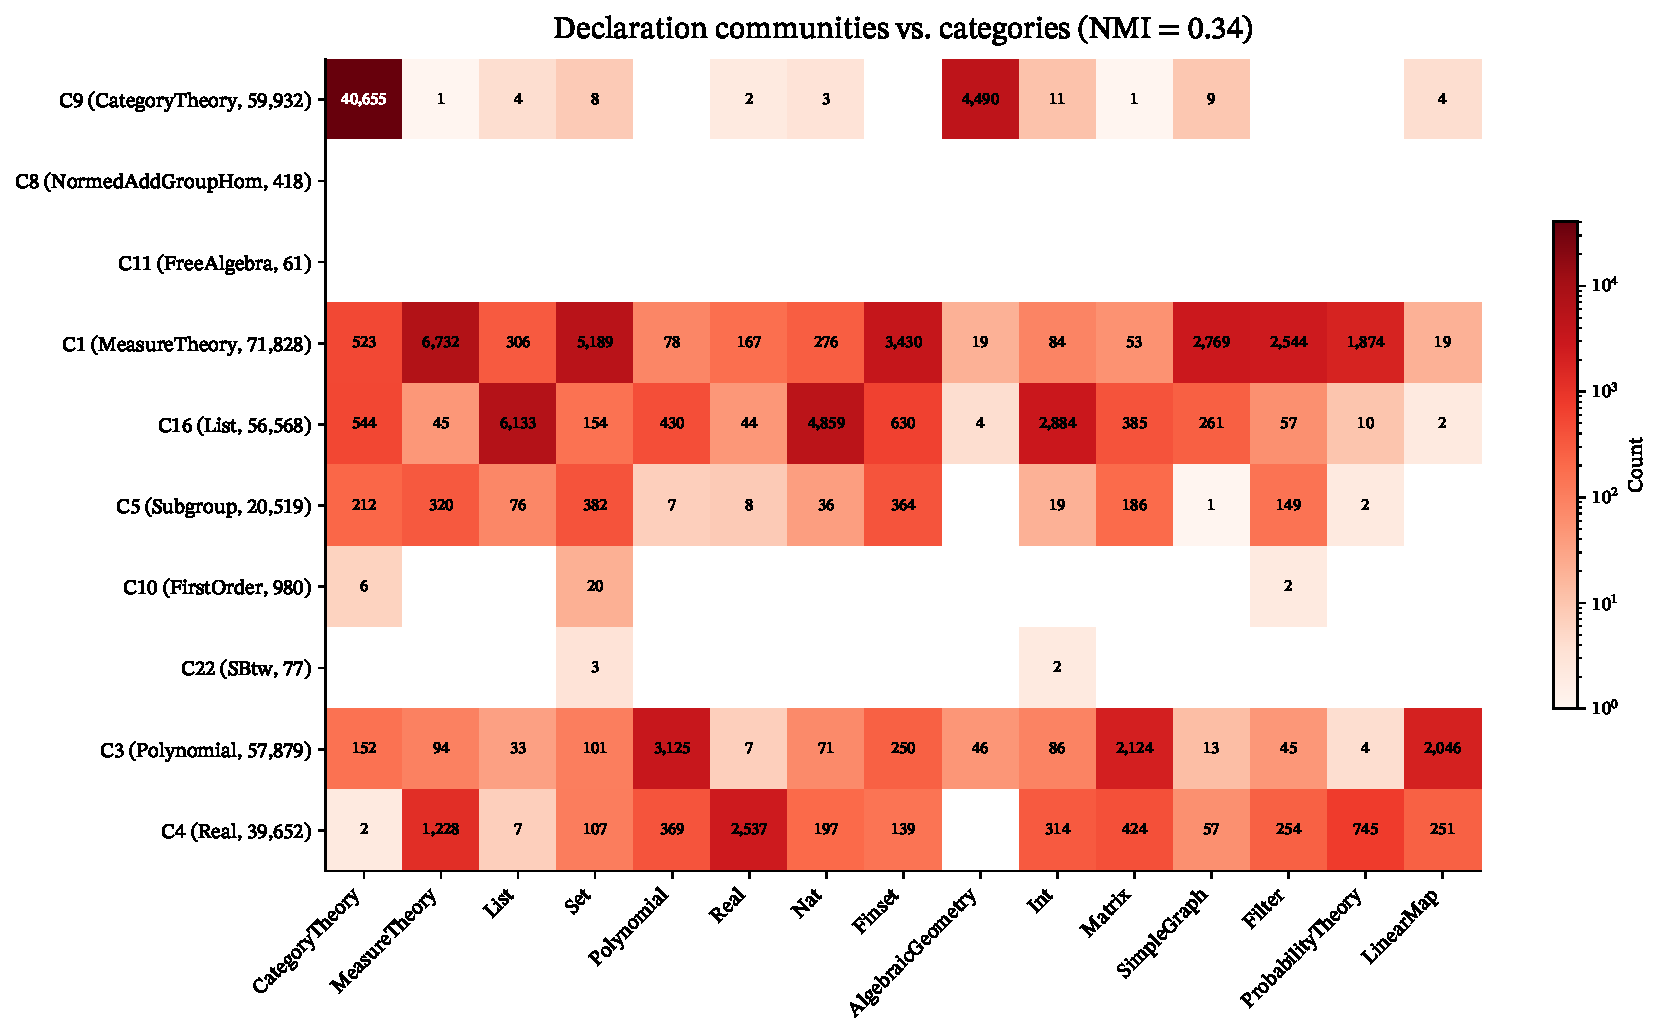
\includegraphics[width=\textwidth]{figures/community_decl_heatmap.pdf}
\caption{Community$\,\times\,$namespace membership heatmap for $G_{\mathrm{thm}}$ (NMI~$= 0.35$, log scale). \ns{CategoryTheory} (C32) concentrates sharply in one cell; the largest community is spread across every column, functioning as a ``catch-all'' with no dominant namespace.}
\label{fig:community-decl-heatmap}
\end{figure}

\subsubsection{Robustness}
\label{sec:thm-robustness}

We assess the resilience of $G_{\mathrm{thm}}$ under two node-removal strategies: random removal and targeted removal in order of decreasing PageRank.

\paragraph{Single-node removal.} Removing any one of the top-$30$ PageRank nodes has negligible impact on connectivity. The largest effect is the removal of \decl{Eq.refl}, which disconnects exactly $6$ of $308{,}054$ nodes from the giant component ($0.002\%$). No single declaration is a critical point of failure. This contrasts with the module-level finding (Table~\ref{tab:robustness}), where removing the top-$5$ modules fragments $G_{\mathrm{module}}$ into $29$ components. The difference arises because module-level removal is coarser: removing a module removes all declarations it contains, severing many edges simultaneously. At the theorem level, each declaration is individually expendable.

\paragraph{Progressive removal.} Under progressive node removal, the asymmetry between random and targeted attack becomes apparent.

\begin{table}[ht]
\centering
\caption{Robustness of $G_{\mathrm{thm}}$ under progressive node removal. The table reports the fraction of nodes remaining in the largest weakly connected component.}
\label{tab:thm-robustness}
\begin{tabular}{rrrl}
\toprule
Removal \% & Random & Targeted & Gap \\
\midrule
$1\%$  & $0.990$ & $0.975$ & $0.015$ \\
$5\%$  & $0.950$ & $0.868$ & $0.082$ \\
$10\%$ & $0.899$ & $0.722$ & $0.177$ \\
$15\%$ & $0.849$ & $0.583$ & $0.266$ \\
$20\%$ & $0.799$ & $0.461$ & $0.338$ \\
\bottomrule
\end{tabular}
\end{table}

\begin{figure}[ht]
\centering

\includegraphics[width=0.85\textwidth]{figures/thm_robustness_curve.pdf}
\caption{Robustness curves for $G_{\mathrm{thm}}$: fraction of nodes in the largest WCC as a function of the fraction removed, under random removal (indigo) and targeted removal by PageRank (gold).}
\label{fig:thm-robustness}
\end{figure}

Under random removal, the giant component shrinks almost linearly---removing $20\%$ of nodes leaves $80\%$ connected. Under targeted attack (removing the highest-PageRank nodes first), $20\%$ removal reduces connectivity to $46\%$---a $34$-percentage-point gap. This is the classic signature of a hub-dominated network~\cite{albert2000,barabasi1999}: resilient to random failure, vulnerable to targeted attack on hubs.

\noindent\textbf{Note.}
\label{rem:thm-robustness-redundancy}
The extreme resilience to single-node removal at the theorem level---no single declaration is a critical bridge---has a deeper explanation than mere edge density. It reflects the inherent \emph{logical redundancy} of mathematical proof. The same lemma is typically reachable through multiple independent proof paths: \decl{Eq.refl} can be circumvented via \texttt{rfl}, \decl{Eq.mpr}, or tactic-generated proof terms; a group-theoretic fact can be accessed through the group axioms or through the ring axioms that subsume them. This redundancy is not engineered (unlike the module-level redundancy of umbrella imports discussed in \S\ref{sec:transitive-reduction}); it is an intrinsic property of mathematical logic. The product carries its own structural insurance.

\subsubsection{Theorem vs.\ Lemma: Validating Human Importance Judgments}
\label{sec:thm-vs-lemma}

In Lean~4 source code, developers choose between \texttt{theorem} and \texttt{lemma} to declare propositions. While the kernel treats both identically---\texttt{lemma} is syntactic sugar for \texttt{theorem}---the choice carries cognitive significance: \texttt{theorem} typically marks a major result, while \texttt{lemma} signals an auxiliary stepping stone. Our extraction pipeline records both as kind \texttt{theorem}, erasing this distinction.

To recover it, we parsed the \module{Mathlib} source code, tracking \texttt{namespace} blocks to reconstruct fully qualified names, and cross-referenced with~$G_{\mathrm{thm}}$.\xinze{LeanScout pipeline: could cross-validate} Of the $251{,}642$ propositions in the graph, $175{,}567$ ($69.8\%$) were matched to a source declaration: $129{,}444$ marked \texttt{theorem} and $46{,}123$ marked \texttt{lemma}.

\begin{table}[ht]
\centering
\begin{tabular}{lccc}
\toprule
Metric & \texttt{theorem} & \texttt{lemma} & Ratio \\
\midrule
Mean in-degree        & $5.16$ & $3.52$ & $1.47\times$ \\
Zero-citation rate    & $37.2\%$ & $39.4\%$ & --- \\
Mean PageRank         & $7.52 \times 10^{-7}$ & $6.83 \times 10^{-7}$ & $1.10\times$ \\
\bottomrule
\end{tabular}
\caption{Structural comparison of declarations marked \texttt{theorem} vs.\ \texttt{lemma} in source code. All three metrics confirm that human importance judgments align with topological prominence.}
\label{tab:thm-vs-lemma}
\end{table}

All three metrics confirm that human importance judgments are validated by the logical structure: declarations that developers considered major results do occupy more prominent positions in the dependency network. The effect is moderate---a $1.47\times$ ratio in citation count, not an order-of-magnitude difference---suggesting that the theorem/lemma boundary is a noisy but genuine signal of structural importance.

\noindent\textbf{Misjudged importance.}
\label{rem:misjudged}
The alignment is imperfect. Among the notable outliers: \decl{funext} (function extensionality) is marked \texttt{lemma} in source code but has in-degree $15{,}574$, making it one of the most cited propositions in \module{Mathlib}. Conversely, $48{,}177$ declarations marked \texttt{theorem}---over a third of all matched theorems---have zero citations. The former represents underestimation of structural importance by the author; the latter represents overestimation, or more precisely, the distinction between importance as a mathematical result (worthy of the name ``theorem'') and importance as a dependency hub (actually reused by other proofs). In the language of our framework, the theorem/lemma distinction is a trace of the process---a record of the author's cognitive judgment at the time of writing---that the product partially but not fully corroborates.
